%%%%%%%%%%%%%%%%%%%%%%%%%%%%%%%%%%%%%%%%%%%%%%%%%
%------ LaTeX-Template
%%%%%%%%%%%%%%%%%%%%%%%%%%%%%%%%%%%%%%%%%%%%%%%%%

%---- Header (mit Formateinstellugen) laden, Inputencoding prüfen ------

%%%%%%%%%%%%%%%%%%%%%%%%%%%%%%%%%%%%%%%%%%%%%%%%%
%---- LaTeX-Header
%%%%%%%%%%%%%%%%%%%%%%%%%%%%%%%%%%%%%%%%%%%%%%%%%

\documentclass[12pt,paper=A4,numbers=noenddot,bibliography=totoc,listof=totoc,DIV=11,BCOR=1mm]{scrreprt}
%  Bindekorrektur BCOR (verlorener Rand am linken Blattrand)! Wert haengt von der Art der Heftung ab!!
%  Satzspiegeleinstellung DIV von KOMA-Script / sccreprt.

\pagestyle{headings}

\usepackage[T1]{fontenc} % Font Encoding fuer europaeische Schriften mit Umlauten (Unterstuetzung der Worttrennung)
\usepackage{lmodern} % PostScript-Varianten der TeX Computer Modern-Schriften laden
\usepackage[english,ngerman]{babel} % Spracheinstellungen fuer Englisch und Neudeutsch laden

\usepackage{setspace}

\usepackage{graphicx} % Grafikeinbindung (fuer .JPG, .JPEG, .PNG und .PDF, falls pdflatex benutzt wird)
\usepackage[table]{xcolor} % ermoeglicht farbige Schrift und farbige Tabellenzeilen
\definecolor{black}{gray}{0} % Umdefinition der Farbe black, falls noetig (0=schwarz, 1=weiss)
\definecolor{dblue}{rgb}{0.1,0.2,0.6} % Dunkelblau, fuer Hyperlinks
\definecolor{lgray}{gray}{0.9} % Hellgrau, fuer Tabellen (0=schwarz, 1=weiss)

\usepackage{booktabs} % fuer schoene Tabellen

\usepackage[round,authoryear]{natbib} % Literaturverweise mit Name/Jahreszahl in runden Klammern
\bibpunct[:\,]{(}{)}{,}{a}{}{,~}  % Feinformatierung der Natbib-Zitierweise

\usepackage[hyphens]{url}
\usepackage[colorlinks=true,linkcolor=black,citecolor=dblue,urlcolor=dblue]{hyperref} 
\usepackage{hyperref}  
% die Pakete url und hyperref ermoeglichen anklickbare URLs im Quellenverzeichnis in definierter Farbe, 
% sie ermoeglichen den Zeilenumbruch bei langen URLs, und sie erzeugen Hyperlinks (Farbe s.o.) 
% zwischen Quellenverweis und Quellenverzeichnis sowie zwischen label und ref im PDF-Dokument

\usepackage[section]{placeins}
% Fonteinstellungen fuer Bildunterschriften: Unterschrift serifenlos, "Abbildung" fett (bfseries = bold face series)
\setkomafont{captionlabel}{\sffamily\bfseries}
\setkomafont{caption}{\sffamily}

%------------------------------------------------------------------------------------------------------------------
%------ Eigenstaendigkeitserklaerung im gerahmten Kasten (parbox in einer framebox) ------
%------------------------------------------------------------------------------------------------------------------

\newcommand{\eigen}{
\setlength{\fboxsep}{2ex}
\setlength{\fboxrule}{0.8pt} 
% Einstellungen fuer Rahmenabstand und Rahmendicke der Framebox
\begin{center}
	\fbox{
		\parbox{0.8\linewidth}{
		Ich versichere, die vorliegende Arbeit selbstst\"andig ohne fremde Hilfe verfasst 
		und keine anderen Quellen und Hilfsmittel als die angegebenen benutzt zu haben. 
		Die aus anderen Werken w\"ortlich entnommenen Stellen oder dem Sinn nach 
		entlehnten Passagen sind durch Quellenangaben eindeutig kenntlich gemacht.
		\par\bigskip\bigskip\bigskip\bigskip
		\hspace*{0.8cm}Ort, Datum \hfill \vorname~\nachname\hspace*{0.8cm}
		}
	}
\end{center}
}

%%%%%%%%%%%%%%%%%%%%%%%%%%%%%%%%%%%%%%%%%%%%%%%%%

%\usepackage[applemac]{inputenc} % Inputencoding f�r Mac
%\usepackage[latin1]{inputenc} % Inputencoding f�r PC/Win
\usepackage[utf8]{inputenc} % Inputencoding, universell
%\usepackage[utf8x]{inputenc} % Inputencoding, universell


%------------------------ Titelblatt-Layout laden ----------------------------------

%%%%%%%%%%%%%%%%%%%%%%%%%%%%%%%%%%%%%%%%%%%%%%%%%
%------ LaTeX-Titelblatt
%------ Deklarationen fuer die Titelseite
%%%%%%%%%%%%%%%%%%%%%%%%%%%%%%%%%%%%%%%%%%%%%%%%%

\title{\titel\\[2ex]
\LARGE Bachelor-Thesis\\
\large zur Erlangung des akademischen Grades B.Sc.\\[1.5ex]
\LARGE \vorname~\nachname\\[0.5ex] 
\large \matrikelnummer
}

\author{\unitlength1mm
\large\raisebox{-1ex}{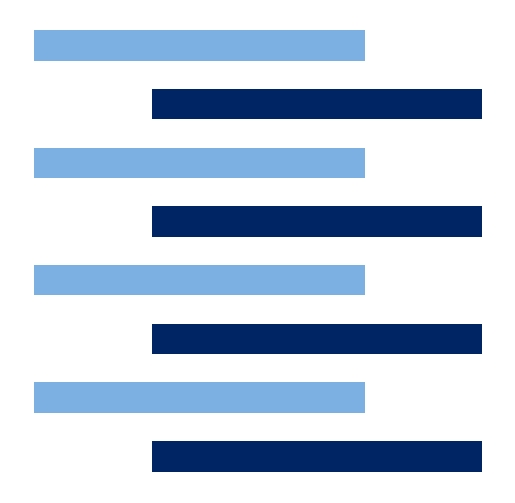
\includegraphics[width=4em]{HAW_wuerfel}}\hspace{1ex}
\parbox[b]{11.2cm}{\sffamily\large%
Hochschule für Angewandte Wissenschaften Hamburg\\[-0.2ex]
Fakultät Design, Medien und Information\\[-0.2ex]
Department Medientechnik
}\\[6ex]
\sffamily\large Erstprüfer: \erstpruef\\[0.5ex]
\sffamily\large Zweitprüfer: \zweitpruef}

%%%%%%%%%%%%%%%%%%%%%%%%%%%%%%%%%%%%%%%%%%%%%%%%%

%---------------------------- Titeldefinitionen --------------------------------------

\newcommand{\vorname}{Sebastian}
\newcommand{\nachname}{Bohn}
\newcommand{\matrikelnummer}{2036605}

\newcommand{\titel}{Analyse und Evaluierung von plattformübergreifenden Spiel-Engines und Frameworks,anhand der Implementierung einer mobilen Beispielapplikation}

\newcommand{\erstpruef}{Prof. Dr. Edmund Weitz}
\newcommand{\zweitpruef}{Prof. Dr. Andreas Plaß}

\date{vorläufige Fassung vom \today}   % Vorab-Version 
%\date{\sffamily Hamburg, DD. MM. YYYY}  % Abgabedatum!

%----------------------------- ANFANG --------------------------------------

\begin{document}
\selectlanguage{ngerman}
\setlength{\parindent}{0em}
% Titelseite erzeugen
\maketitle
% Inhaltsverzeichnis erzeugen          
\tableofcontents
% Seitenumbruch
\clearpage

%----------------------------INHALT---------------------------------------

%---------------------------ABSTRACT------------------------------------

\thispagestyle{empty}
\selectlanguage{english}
\section*{\centering\abstractname}

%TODO: English abstract

\selectlanguage{ngerman}
\section*{\centering\abstractname}

%TODO: Deutsches abstract

%----------------------------TEXT-----------------------------------------------

%TODO: Kapitel 1
\chapter{Einleitung}

\section{Motivation}
\section{Gliederung}

%Kapitel 2
\chapter{Mobile Systeme}

\section{Marktanalyse zur Gewichtung der mobilen Systeme und der Applikationen}
Welche mobilen Systeme derzeit am meisten gefragt und verbreitet sind, soll in diesem Abschnitt analysiert werden. Dieses Wissen ist nötig, um vor dem Entwicklungsprozess die erfolgreichsten und erfolgversprechendsten Plattformen auszuwählen und miteinzubeziehen.
Weiterhin soll geklärt werden wie viele Applikationen diese Plattformen in ihren Stores bereitstehen und wie die Kategorien gewichtet sind.

\subsection{Marktanteile an mobilen Betriebssysteme}
\label{subsec:Marktanteile_mobile_Systeme}
Eine Statistik über die Marktanteile der mobilen Betriebssysteme bei Smartphones, soll veranschaulichen welche Systeme aktuell zu den führenden gehören. Zusätzlich wird eine zukünftige Verteilung prognostiziert. Die Darstellungen beziehen sich auf Daten der International Data Corporation (IDC), über den globalen Absatz von Smartphones und wurde im August 2015 veröffentlicht. (Abb. \ref{graph_mobile_systems})

\begin{figure}[htbp]
	\centering
	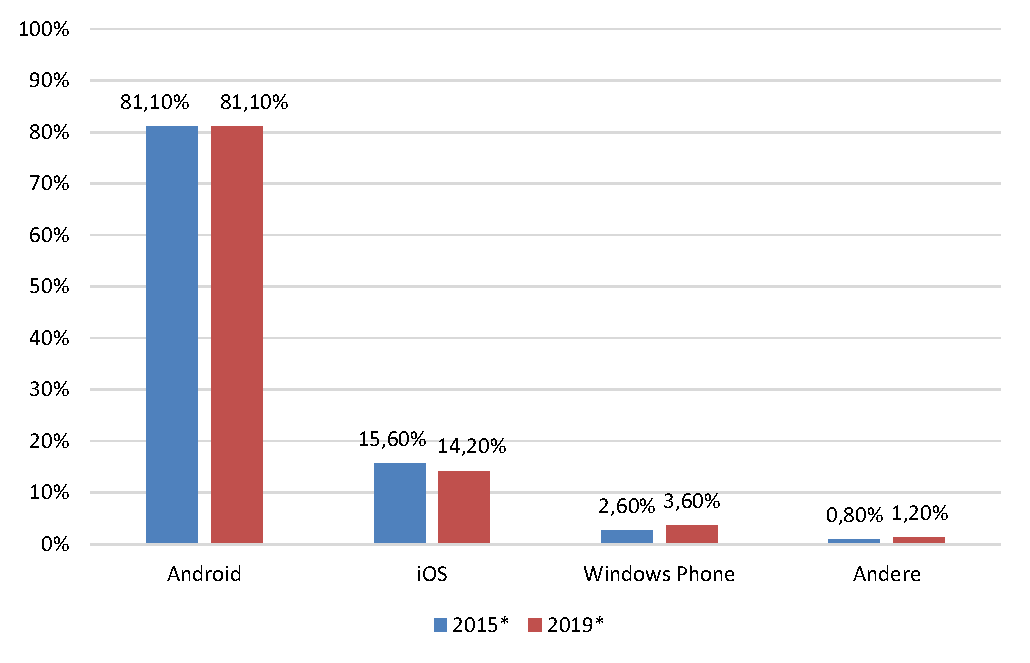
\includegraphics[width=0.8\textwidth]{Bilder/Marktanteile_Betriebssysteme}
	\caption{Prognose zu den Marktanteilen der Betriebssysteme am Absatz vom Smartphones weltweit in den Jahren 2015 und 2019}\label{graph_mobile_systems}\citep{marktanteile_betriebssysteme}
\end{figure}

Die Grafik verdeutlicht, dass aktuell Geräte mit Android Systemen den Markt eindeutig dominieren. Darauf folgen Geräte mit iOS und Windows Phone. Laut Prognose wird sich auch in den nächsten Jahren an dieser Hierarchie nichts ändern. Schlussfolgernd sind diese drei Systeme die relevantesten auf dem globalen Markt.

Abbildung \ref{graph_mobile_systems_laender} gibt Aufschluss über die Verteilung der Systeme nach ausgewählten Ländern. Die Daten beziehen sich auf die Verkäufe von August bis Oktober 2015, welche von Kantar im Dezember 2015 veröffentlicht wurden. Bei der Internationalisierung von Applikationen ist es von Vorteil zu wissen, wie stark die Gewichtung der Systeme in den einzelnen Ländern ist.

\begin{figure}[htbp]
	\centering
	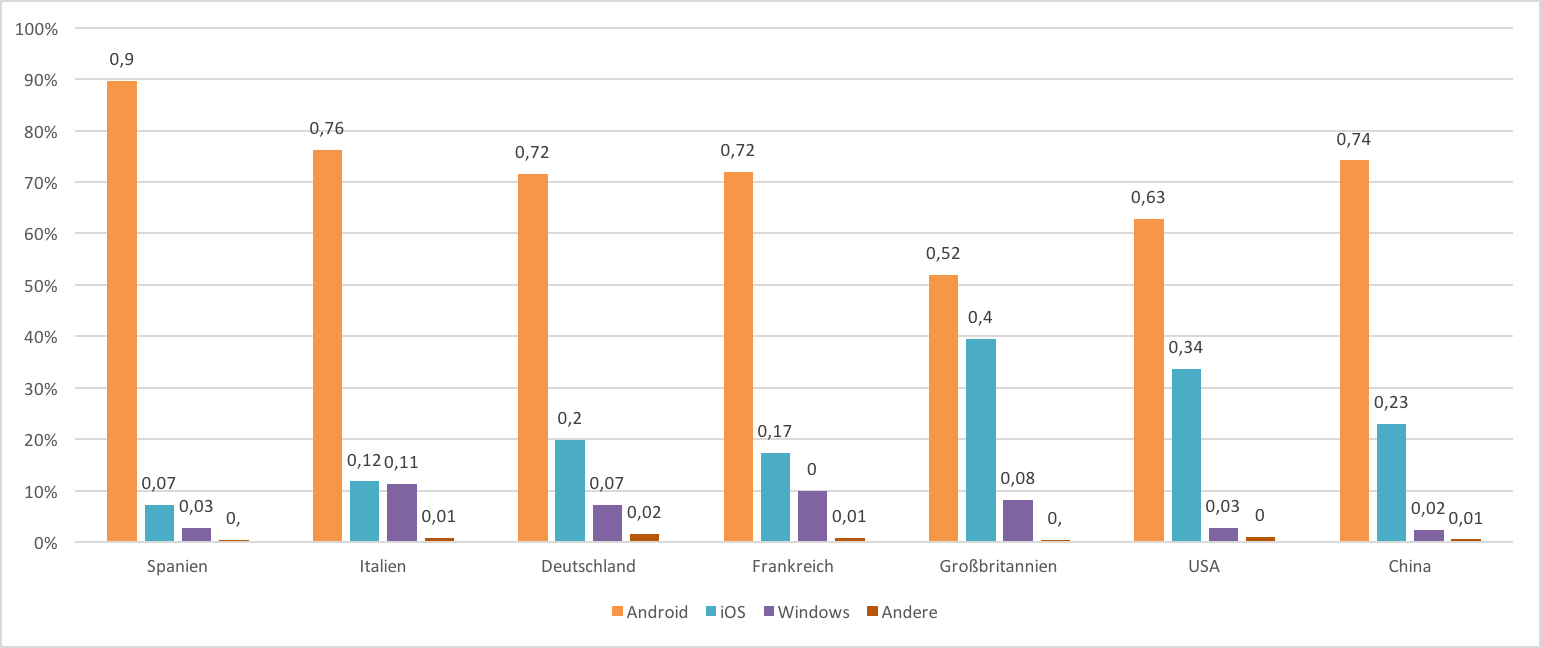
\includegraphics[width=0.8\textwidth]{Bilder/Marktanteile_nach_Laendern}
	\caption{Marktanteile der mobilen Betriebssysteme am Absatz von Smartphones in ausgewählten Ländern von August bis Oktober 2015}\label{graph_mobile_systems_laender}\citep{marktanteile_betriebssysteme_laender}
\end{figure}

\subsection{Verfügbare Applikationen und Kategorien der Stores}
Die Menge an verfügbaren Apps in den jeweiligen Stores ist unterschiedlich groß.
Eine Analyse über die aktiven Applikationen in den einzelnen Stores und die Gewichtung der Kategorien, soll einen Überblick verschaffen was die jeweiligen Plattformen aktuell zu bieten haben.
In Abbildung \ref{graph_apps_in_stores} wird die Menge an verfügbaren Apps im Mai 2015 dargestellt. Um eine bessere Übersicht zu gewährleisten, wurden die Werte gerundet. Der Amazon Appstore bietet wie der Google Play Store nur Android Apps an. Da es in diesen beiden Stores zum Teil zu Überschneidungen beim Angebot von Anwendungen kommt, werden diese Werte separat betrachtet und nicht summiert.

\begin{figure}[htbp]
	\centering
	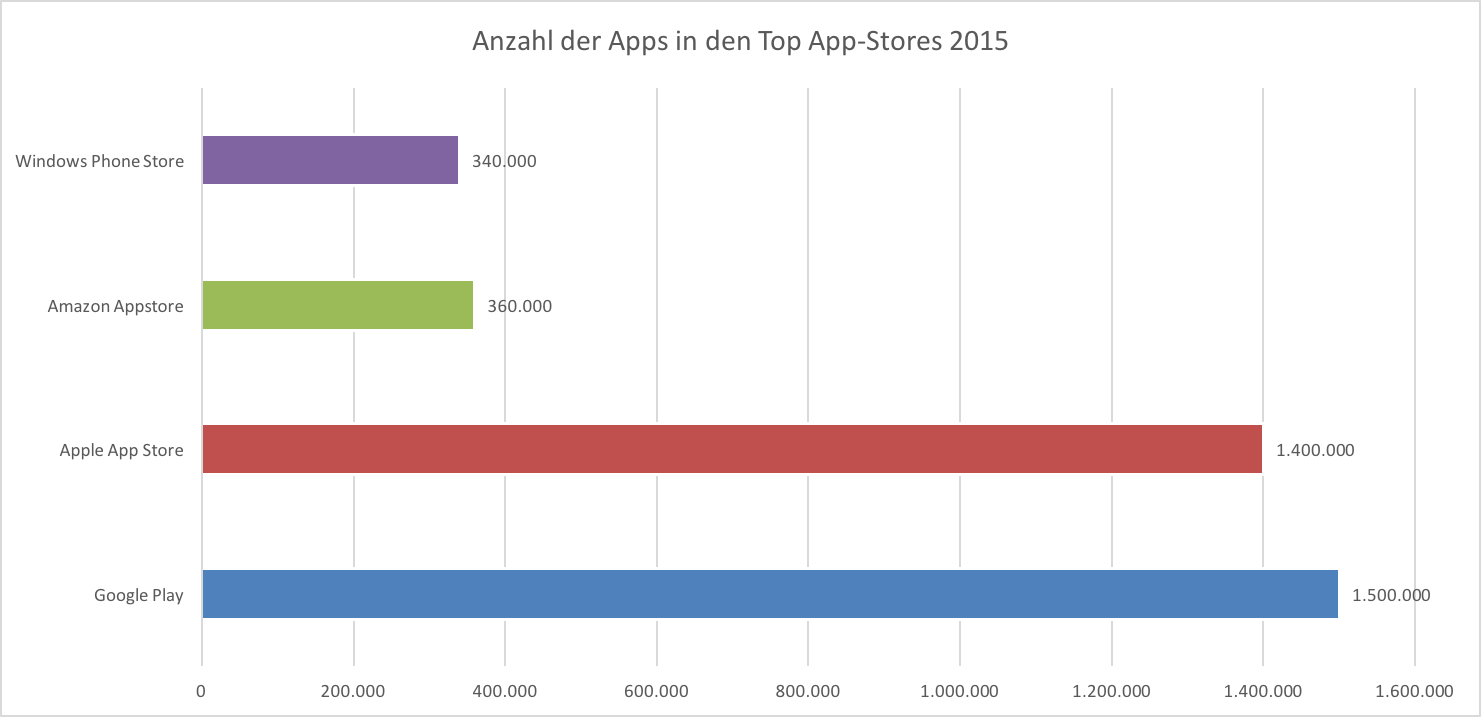
\includegraphics[width=0.8\textwidth]{Bilder/Anzahl_der_Apps}
	\caption{Anzahl der angebotenen Apps in den Top App-Stores im Mai 2015}\label{graph_apps_in_stores}\citep{apps_in_stores}
\end{figure}

Der Wert für den Windows Phone Store ist der Quelle nach von September 2014 und schließt damit noch nicht die Windows 10 Universal Apps mit ein. Diese kamen erst Mitte 2015 dazu und werden in einem getrenntem Windows Store hardwareübergreifend angeboten. Im September 2015 waren rund 80\% der Downloads aus dem Windows Phone Store von Geräten mit der Version 8.1, etwa 15\% von 8.0 Benutzern und etwa 5\% von der aussterbendem Version 7.8.
Laut Windows wurden im September 2015 etwa 50\% der Applikationen mit Windows 10 aus dem neuen Windows Store heruntergeladen. Diese Statistik gibt jedoch wenig Aufschluss wie groß dabei der Anteil an mobilen Systemen ist. Jedoch dominiert die Kategorie "Games" bei Windows 10 Apps mit fast 45\% die Downloadzahlen.\citep{windows_store_trends_2015}

\begin{figure}[htbp]
	\centering
	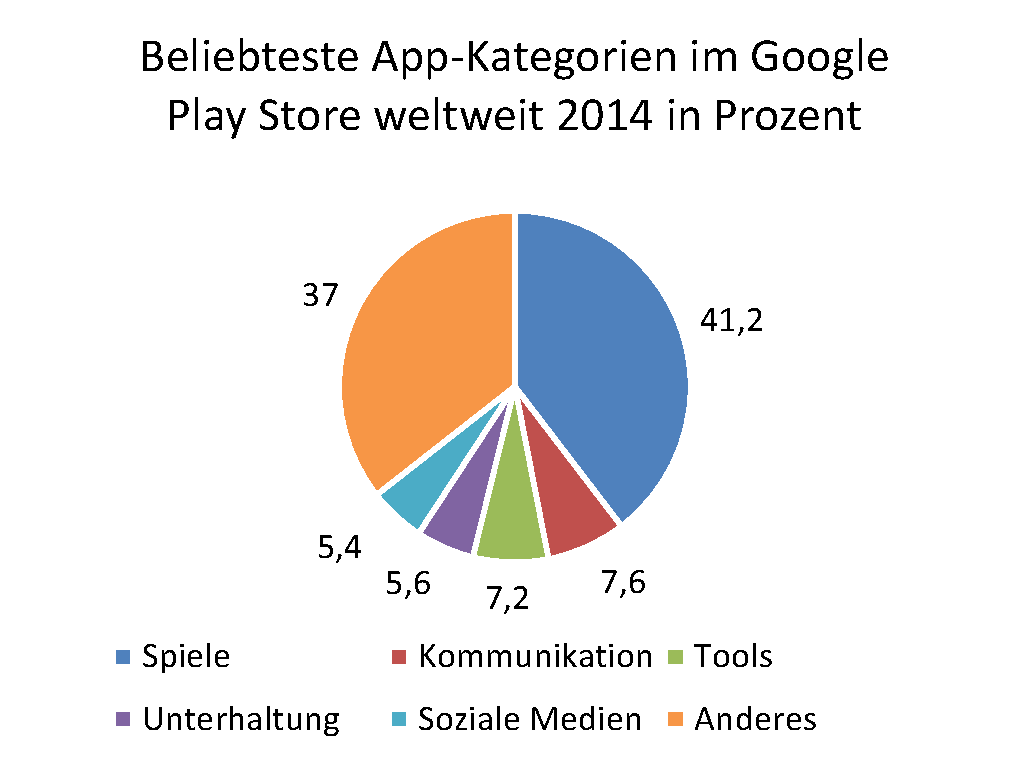
\includegraphics[width=0.8\textwidth]{Bilder/Google_Play_Store_Kategorien}
	\caption{Anteil der im Google Play Store weltweit am häufigsten heruntergeladenen Apps nach Kategorien im Februar 2014}\label{graph_play_store_kategorien}\citep{play_store_categories}
\end{figure}

Auch im Google Play Store werden Spiele Apps am häufigsten heruntergeladen und nehmen etwa 41\% des Downloadvolumens ein.(Abb.\ref{graph_play_store_kategorien})

\begin{figure}[htbp]
	\centering
	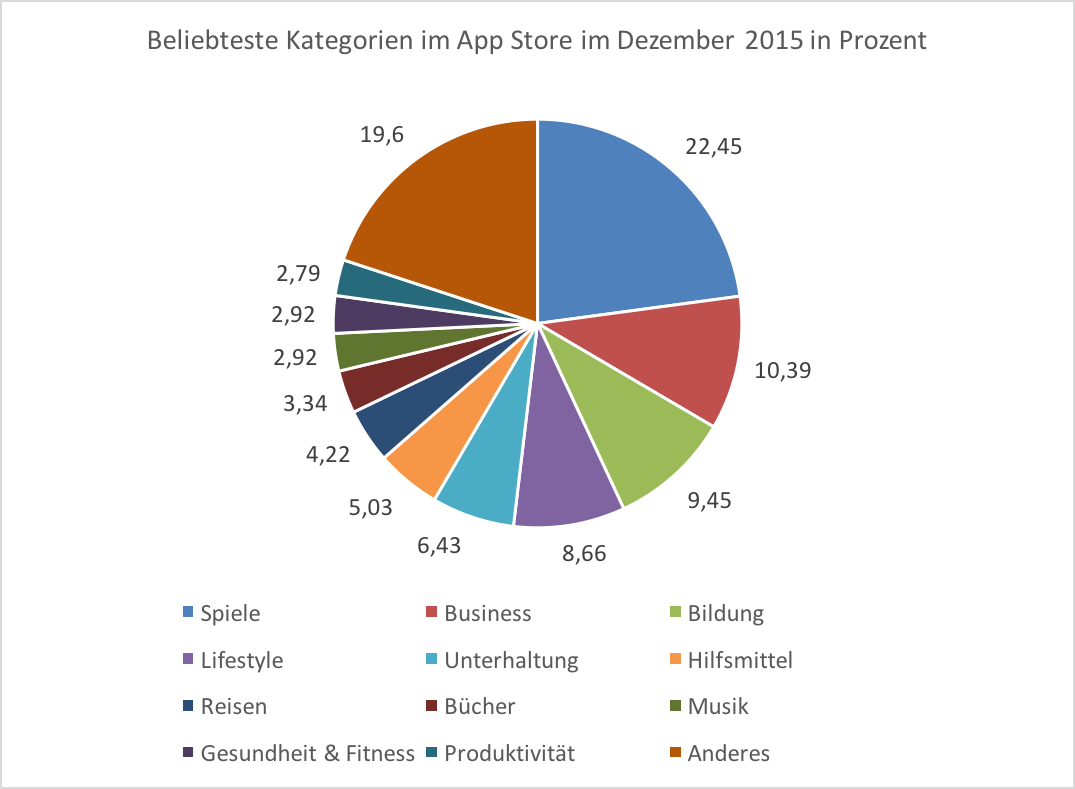
\includegraphics[width=0.8\textwidth]{Bilder/Top_Kategorien_App_Store}
	\caption{Ranking der Top-Kategorien im App Store im Dezember 2015}\label{graph_app_store_kategorien}\citep{app_store_categories}
\end{figure}

Die beliebtesten Kategorien des Apple App Store werden ebenfalls deutlich von den Spielen angeführt. Auch wenn der Abstand zur zweithäufigsten Kategorie geringer ist als bei den anderen Stores, macht der Spielebereich trotzdem etwa ein viertel aller Downloads aus.(Abb.\ref{graph_app_store_kategorien})
\medskip

Auch wenn jeder Store seine Applikationen auf eigene Weise kategorisiert, ist dennoch klar zu erkennen das Spiele bei jedem Anbieter das höchste Downloadvolumen ausmachen und sich stetig wachsender Beliebtheit erfreuen. Die Nachfrage nach mobilen Spielen ist demnach plattformübergreifend und berechtigt die Evaluierung von entsprechender Entwicklungssoftware.

\section{Betrachtung der mobilen Systeme}
Anhand der gewonnenen Erkenntnisse aus Kapitel \ref{subsec:Marktanteile_mobile_Systeme}, spielen derzeit die mobilen Systeme von Android, iOS und Windows Phone die größte Rolle auf dem Markt und bei den Benutzern. Folglich werden weitere Systeme nicht weiter betrachtet und der Fokus auf diese drei Systeme gerichtet.

\subsection{Android}
Android ist ein Open Source Betriebssystem und gleichzeitig eine Software-Plattform, welches stark im mobilen Bereich vertreten ist und auf dem Linux-Kernel basiert. Zu finden ist diese auf Smartphones, Tablet-Computern, Netbooks und auch auf Smart-TV Geräten. \citep{android_overview} Entwickelt wird Android von der Open Handset Alliance (OHA), welche von Google gegründet wurde. Die OHA wurde im November 2007 gegründet und ist ein Konsortium von mehr als 80 Unternehmen aus den Bereichen Mobilfunknetz, Geräteherstellung, Halbleiterindustrie, Marketing und Software. \citep{alliance_members} Der Grund für die Entwicklung von Android war und ist es, einen offenen Standard für mobile Geräte zu schaffen. \citep{alliance_overview}

Durch seine Offenheit ermöglicht Android Entwicklern große Freiheit bei der Programmierung von Applikationen. Eigene Entwicklungen können auch mit Anwendungen von Google, wie zum Beispiel Google Maps, verknüpft werden.

Auch der Hardwarebereich bietet ein breites Spektrum an Geräten mit kostengünstigen, bis hochpreisigen Angeboten, sowohl mit einfacher bis qualitativ hochwertiger, technischer Ausstattung. Benutzer haben die Möglichkeit, ihre Geräte weitestgehend frei zu gestalten und einzustellen. Für die Installation von neuen Applikationen sind diese auch nicht an einen einzigen Store gebunden und können Apps auch aus verschiedensten Quellen beziehen.
\\

Vorteile:
\begin{itemize}
	\item Open Source
	\item Unabhängigkeit von Anbietern
	\item Personalisierung
	\item Hardwareangebot
\end{itemize}

Nachteile:
\begin{itemize}
	\item Hohe Verbreitung von Schadsoftware
	\item Aktualität der Version ist abhängig vom Gerätehersteller
\end{itemize}

\subsection{iOS}
iOS ist das mobile Betriebssystem des Unternehmen Apple. Dieses ist ein Derivat von Mac OS X, welches selbst auf Unix basiert. Es wird ausschließlich von Apple entwickelt und ist somit nur auf den eigenen Geräten iPhone, iPad und iPod touch zu finden. Mit der Entwicklung wurde unter externer und interner Geheimhaltung 2005 begonnen und das Resultat der Öffentlichkeit zum ersten Mal Anfang 2007 vorgestellt. Bis zur Version 4.0 wurde iOS mit dem Namen iPhoneOS betitelt. Das Konzept und Design ist schwerpunktmäßig auf hohe Benutzerfreundlichkeit und Funktionalität ausgelegt. 

Durch die geschlossene Struktur des Systems sind eigene Derivate nicht möglich. Benutzer sind für den offiziellen Bezug von Applikationen auf Apples App Store angewiesen.
Bei der Wahl der Hardware ist man auf die Produktpalette von Apple angewiesen, welche jährlich eine neue Generation veröffentlicht. Die Personalisierung der Geräte ist nur bedingt möglich, da Anbieter von Drittsoftware keinen Zugriff auf das System haben und Anwendungen nur offiziell über den eigenen App Store bezogen werde können. Dies bietet jedoch den Vorteil einer Qualitätssicherung durch Apple, da Applikationen vor der Veröffentlichung einer Prüfung unterzogen werden.
\\

\textbf{Vorteile:}
\begin{itemize}
	\item Kompatibilität von Software und Hardware
	\item Benutzerfreundlichkeit
	\item Geräteübergreifende Kommunikation
	\item Kontrollen bei Veröffentlichung von Anwendungen
\end{itemize}

\textbf{Nachteile:}
\begin{itemize}
	\item Restriktive Firmenpolitik
	\item Proprietäres System
	\item Hardwareauswahl
	\item Anwendungen nur über den App Store
\end{itemize}

\subsection{Windows Phone}
Entwickler Microsoft stellt seit dem Jahr 2000 Betriebssysteme für mobile Geräte her. \citep{microsoft_mobile} 
Seitdem hat sich die Namensgebung von Windows Mobile, über Windows Phone, bis zum aktuellsten Windows 10 Mobile vorgearbeitet. Um im allgemeinen Bezug nicht zwischen den Namen hin und her zu wechseln, wird in dieser Arbeit, wenn mobile Windows Systeme erwähnt werden, der Name Windows Phone benutzt.
Die frühen Versionen von Windows Phone, also Windows Mobile und Windows Phone 7 stammen noch von dem Windows CE Kernel ab, wobei die aktuellen Versionen, Windows Phone 8 und Windows 10 Mobile, Derivate des Windows NT Kernels sind. Mit dem neuesten Ableger, Windows 10 Mobile, verspricht Microsoft eine homogene Kommunikations- und Anwendungsstruktur zwischen allen Geräten die mit diesem System betrieben werden. Dazu zählen nicht nur Smartphones und Tablets, sondern auch Notebooks, Desktop PCs und die Spielkonsole Xbox One. \citep{windows10_features}

Microsoft verfolgt mit Windows Phone eine ähnlich geschlossene und proprietäre Struktur wie der Konkurrent Apple. Eigene Derivate des Systems sind also nicht offiziell möglich. Auch die Benutzer müssen für neue Anwendungen auf das Angebot des Windows Stores zurückgreifen. Jedoch will Microsoft Entwicklern die Möglichkeit bieten, zukünftige Anwendungen universell verfügbar zu machen, das diese auf allen Windows Systemen nutzbar sind. Microsoft arbeitet außerdem an einer Technik, die bestehende Android und iOS Anwendungen auf die Windows Plattform überführen kann. \citep{wp_with_android_ios}

Die aktuellen Windows Phone Versionen sind durch eine Allianz von Windows und Nokia, hauptsächlich auf mobilen Geräten von Nokia zu finden.\citep{microsoft_nokia}
Aber auch andere Hersteller bieten Geräte mit Windows Phone, jedoch bisher in einem überschaubaren Umfang.
\\

Vorteile:
\begin{itemize}
	\item Kompatibilität von Software und Hardware
	\item Universelle Anwendungen
	\item Benutzerfreundlichkeit
\end{itemize}

Nachteile:
\begin{itemize}
	\item Proprietäres System
	\item Anwendungen nur aus dem Windows Store
	\item Geringeres Angebot an Anwendungen
\end{itemize}
\citep{wp_pros_cons}

%OPTIONAL!!!
%subsection{Weitere Systeme}

%TODO: Kapitel 3
\chapter{Native Softwareentwicklung}
Softwareentwicklung für ein bestimmtes System wird als nativ (lat.: angeboren, natürlich) bezeichnet. Hier sind Dateiformate, Programmiersprachen, Hardware, Entwicklungsumgebungen und Kompilierung genau an die Zielplattform angepasst. Nativer Code ist in der Lage alle individuellen Eigenschaften einer Zielplattform anzusprechen, ohne dabei eine eventuelle Portierbarkeit zu berücksichtigen.
\citep{native_software}
Welche Anforderungen iOS, Android und Windows Phone bezüglich nativer Entwicklung voraussetzen, soll in diesem Kapitel näher erläutert werden.

\section{Systemvorraussetzungen}
Um Applikationen für eine bestimmte Zielplattform zu entwickeln, werden unter Umständen Voraussetzungen an das Betriebssystem des Entwicklers gestellt.

\subsection{iOS}
%TODO

\subsection{Android}
Die Entwicklung von Android Applikationen ist an kein bestimmtes System gebunden. Somit lassen sich diese unter Windows, OS X und Linux Systemen entwickeln. 
Windows Benutzer sollten mindestens Windows XP nutzen. Darüber hinaus können alle aktuelleren Versionen genutzt werden, wobei alle 32-Bit Editionen unterstützt werden und ab Windows 7 auch die mit 64-Bit.
Mac Systeme werden ab OS X 10.5.8 von den offiziellen Entwicklungswerkzeugen unterstützt.
Um auf einem Linux System zu entwickeln, kann man dies beispielsweise unter Ubuntu ab Version 8.04 tun. Bei 64-Bit Versionen ist es notwendig, dass diese fähig ist 32-Bit Anwendungen auszuführen. Da die Auswahl an Linux-Distributionen sehr umfangreich ist, wird an dieser Stelle auf diese nicht weiter eingegangen.
\citep{android_sdk_requirements}

\subsection{Windows Phone}
%TODO

\section{SDKs und Versionen}
Software Development Kits, kurz SDKs, liefern dem Entwickler die Werkzeuge, Anwendungen und bestenfalls eine aktuelle Dokumentation, um für eine bestimmte Zielplattform zu entwickeln. Auch sind sie notwendig, um geschriebenen Code zu interpretieren und kompilieren. Um die aktuellste Version eines mobilen Systems zu unterstützen, muss das SDK auf ebenso aktuellen Stand sein.

\subsection{iOS Versionen}
Apple nutzt für seine Produkte Codenamen, die keinem bestimmten Muster folgen. Verbrauchern sind diese meist unbekannt, da diese überwiegend intern genutzt werden.
\begin{table}[htbp]
\centering
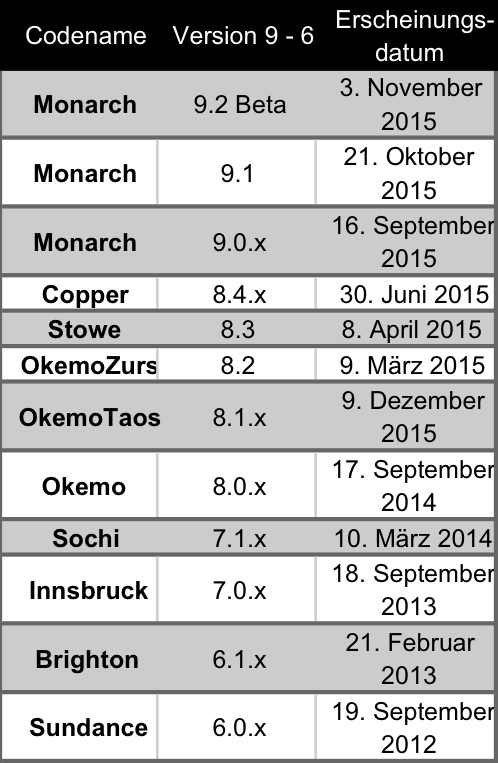
\includegraphics[width=0.5\textwidth]{Tabellen/iOS_Versionen_9-6}
\caption{iOS Versionen 9 - 6 und ihr Erscheinungsdatum}\label{tab_ios_vers_9-6}\citep{ios_codenames}
\end{table}
\begin{table}[htbp]
\centering
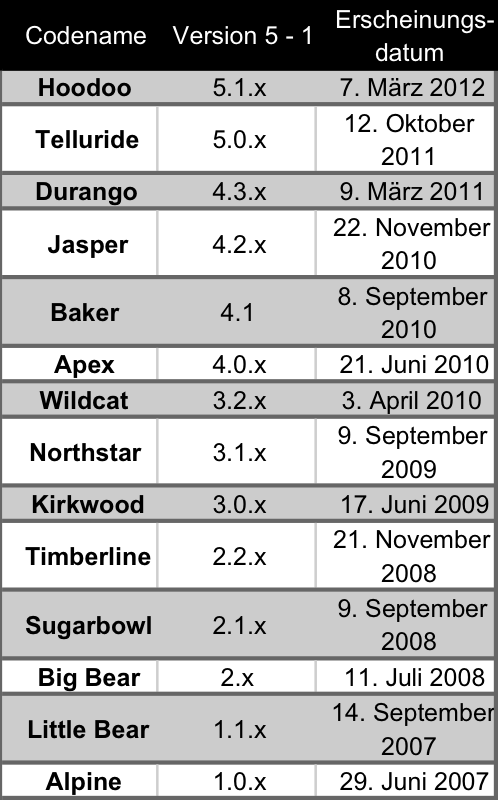
\includegraphics[width=0.5\textwidth]{Tabellen/iOS_Versionen_5-1}
\caption{iOS Versionen 5 - 1 und ihr Erscheinungsdatum}\label{tab_ios_vers_5-1}\citep{ios_codenames}
\end{table}
\clearpage

\subsection{Android Versionen}
Android Versionen sind nach süßen Leckereien benannt und dem Anfangsbuchstaben nach alphabetisch aufsteigend.
\begin{table}[htbp]
\centering
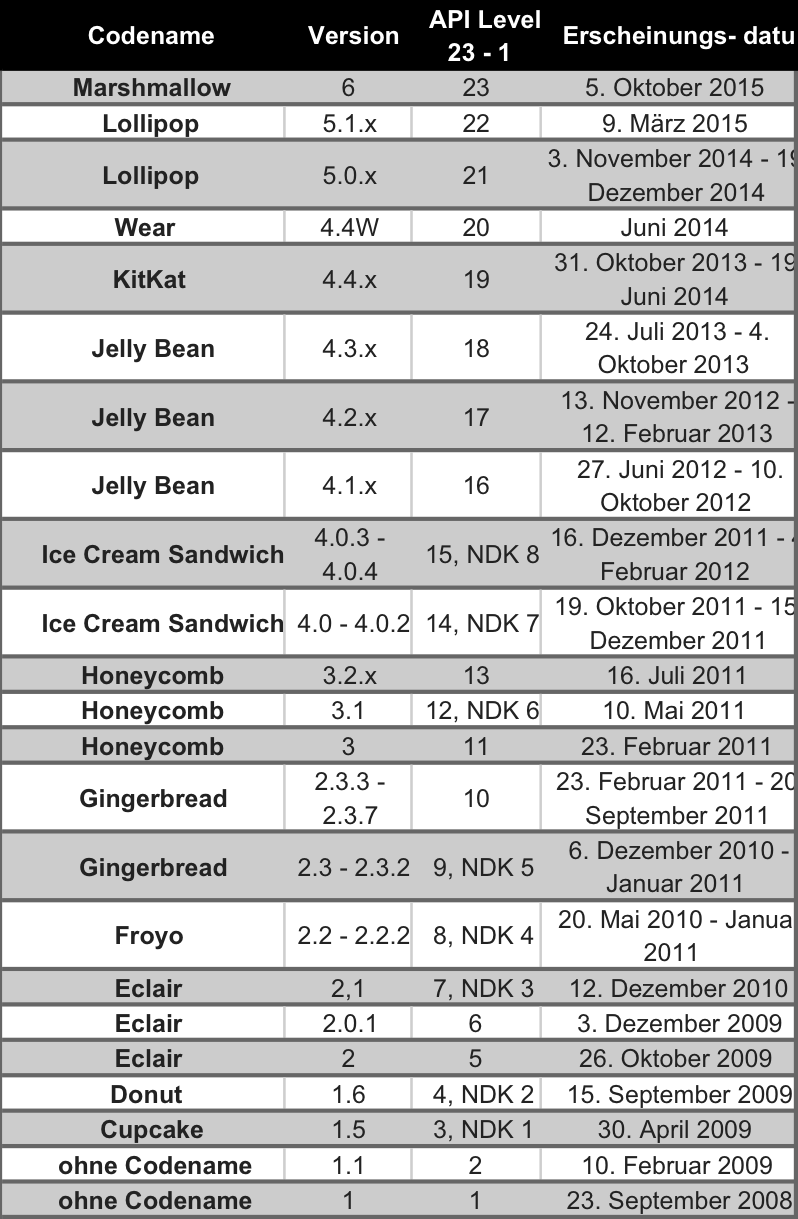
\includegraphics[width=0.6\textwidth]{Tabellen/Android_Versionen}
\caption{Android Versionen und ihr Erscheinungsdatum}\label{tab_android_vers}\citep{android_codenames,android_version_releases}
\end{table}

\clearpage

\subsection{Windows Phone Versionen}
%TODO

\section{Programmiersprachen}
In der nativen Entwicklung werden für jede Zielplattform bestimmte Programmiersprachen unterstützt. 

\subsection{iOS}
%TODO
\subsection{Android}
Android Applikationen werden in Java entwickelt. Demnach ist es notwendig vorab eine aktuelle Java Version (JDK) zu installieren. Diese wird von dem Unternehmen Oracle, mit der aktuellen Version 8 Update 66, vertrieben.
\citep{java_jdk}

\subsection{Windows Phone}
%TODO

%OPTIONAL!!!
%\subsection{Popularität der Programmiersprachen}

\section{Entwicklungsumgebungen}
Für die Entwicklung werden jeweilig verschiedene IDEs (Integrated Development Environment) seitens der Betreiber unterstützt und empfohlen. Eine Besonderheit bei IDEs für mobile Systeme ist die Unterstützung eines Simulators. Dieser simuliert ein spezifiziertes Gerät auf virtuelle Weise, um Entwicklungen direkt testen zu können.

\subsection{iOS}
%TODO
\subsection{Android}
Android empfiehlt das eigene Android Studio, welches die offizielle IDE für Android Entwicklung darstellt und zusätzlich das aktuelle SDK mitliefert. Android Studio basiert auf der IDE IntelliJ IDEA und ist frei verfügbar.\citep{android_studio} Alternativer Vorgänger ist die quelloffene IDE Eclipse.


\subsection{Windows Phone}
%TODO

%OPTIONAL!!!
%\section{Kompilierung}

%OPTIONAL!!!
%TODO: Kapitel 8
%\chapter{Stores für mobile Spiele}
%\section{Allgemeine Bedingungen für Entwickler}
%\section{Maximale App-Größe}
%\section{Anforderungen an den Quellcode}
%\section{Kosten und Abgaben}

%TODO: Kapitel 4
\chapter{Cross-Platform Entwicklung}
\section{Ziel}
\section{Funktionsweise}
\subsection{Technik}
\subsection{Geteilter Content}
\subsection{Übersetzung in die jeweiligen System}

%TODO: Kapitel 5
\chapter{Cross-Platform Frameworks}
\section{Tools und Anbieter zur Entwicklung}
\section{Verweis auf Bachelorarbeit: „Plattformabhängige und –unabhängige Entwicklung mobiler Anwendungen am Beispiel von Geo-Wikipedia-App“}
\section{Gamespezifische Frameworks und Engines}
\subsection{Monogame}
\subsection{Cocos2D}
\subsection{Libgdx}
\subsection{Unity}
\subsection{Unreal Engine}
\subsection{Weitere Frameworks}
\section{Entwicklungsumgebungen}
\subsection{Unterstützte IDEs}
\subsection{Systembedingte Einschränkungen}

%TODO: Kapitel 6
\chapter{Gegenüberstellung der Frameworks}
%Features und Einschränkungen
\section{Zielplattformen}
%\section{Skalierbarkeit der Menge der Plattformen} % ???
\section{Programmiersprachen}
\section{Unterstützung von 2D und 3D}
\section{Zugriff auf Hardware}%Accelerometer etc
\section{Free- und Pro- Versionen}
\section{Einfluss auf Einstellungen}
\section{Zusätzlich benötigte Software}
\section{Aktualität - Versionen - Community}
\section{Zukunftsaussichten}

%OPTIONAL!!!
%TODO: Kapitel 7
\chapter{Analyse der Marktanteile}
\section{Menge an Firmen und Entwicklern}
\section{Menge an Games}

%TODO: Kapitel 9
\chapter{Kosten-Nutzen Vergleich}
%Vergleichstabelle zu den Variationen der Projektanforderungen im Zusammenhang mit den Möglichkeiten und Kosten der Frameworks

%OPTIONAL!!!
%TODO: Kapitel 10
%\chapter{Grundgerüst und Aufbau eines Cross-Plattform Projekts}
%\section{Geteilter Content}
%\section{Plattformabhängiger Content}
%\section{Grundaufbau bei Engines}
%\section{Grundaufbau bei Frameworks}

%OPTIONAL!!!
%TODO: Kapitel 11
%\chapter{Game-typische Design Patterns und Architekturen}
%\section{Architekturen}
%\section{Patterns}
%\section{Verweis auf Bachelorarbeit: „Use of Design Patterns for mobile game Development“}

%OPTIONAL!!!
%TODO: Kapitel 12
%\chapter{Nutzen von Architekturen}
%\section{Pro}
%\subsection{Skalierbarkeit}
%\subsection{Lesbarkeit}
%\subsection{Wiederverwertbarkeit}
%\section{Contra}
%\subsection{KISS - Keep it simple stupid}

%TODO: Kapitel 13
\chapter{Konzeption einer Applikation}
\section{Ideen}
\section{Anforderungen}
\section{User Stories}

%TODO: Kapitel 14
\chapter{Implementierung der Applikation}
\section{Verwendete Frameworks und Engines}
\section{Verwendete APIs und SDKs}
\section{Assets und deren Verwendung}

\chapter{Analyse messbarer Metriken}
%Kosten, Performance, Akkuverbrauch, App-Daten-Aufteilung, Größe des benötigten Speichers, Größe des geteilten Contents, Stabilität, RAM, Code-Zeilen/-Größe, Entwicklungszeit(bedingt zu berücksichtigen)

\chapter{Vergleich der Messprotokolle}

\chapter{Fazit}



%--------------------- VERZEICHNISSE -------------------------------------

\listoffigures % Abbildungsverzeichnis erzeugen
\listoftables % Tabellenverzeichnis erzeugen

%------------------------------ LITERATURVERZEICHNIS----------------------
%TODO:Alphabetisch sortieren!
\begin{thebibliography}{}

\bibitem[Open Handset Alliance - Android Overview(2015)]{android_overview}
\emph{Overview of Android by the Open Handset Alliance},
\url{http://www.openhandsetalliance.com/android_overview.html}, letzter Zugriff: 24.11.2015

\bibitem[Open Handset Alliance - Alliance Overview(2015)]{alliance_overview}
\emph{Overview of the Open Handset Alliance},
\url{http://www.openhandsetalliance.com/oha_overview.html}, letzter Zugriff: 24.11.2015

\bibitem[Open Handset Alliance - Alliance Members(2015)]{alliance_members}
\emph{Members of the Open Handset Alliance},
\url{http://www.openhandsetalliance.com/oha_members.html}, letzter Zugriff: 24.11.2015

\bibitem[Android Source - Codenames, Tags, and Build Numbers(2015)]{android_codenames}
\emph{Codenames, Tags, and Build Numbers in the history of Android},
\url{https://source.android.com/source/build-numbers.html}, etzter Zugriff: 24.11.2015

\bibitem[Wikipedia - Liste von Android-Versionen(2015)]{android_version_releases}
\emph{Übersicht von allen Android Versionen mit Veröffentlichungsdatum},
\url{https://de.wikipedia.org/wiki/Liste_von_Android-Versionen}, letzter Zugriff: 24.11.2015

\bibitem[John Daintith(2004)]{native_software}
\emph{A Dictionary of Computing - native software},
\url{http://www.encyclopedia.com/doc/1O11-nativesoftware.html}, letzter Zugriff: 24.11.2015

\bibitem[Sue Smith(2013)]{android_sdk_requirements}
\emph{Android SDK Requirements},
\url{http://code.tutsplus.com/tutorials/android-sdk-requirements--mobile-20086}, letzter Zugriff: 24.11.2015

\bibitem[the iphone wiki(2015)]{ios_codenames}
\emph{Firmware},
\url{https://www.theiphonewiki.com/wiki/Firmware}, letzter Zugriff: 24.11.2015

\bibitem[Oracle - Java SE(2015)]{java_jdk}
\emph{Java SE Development Kit 8 Downloads},
\url{http://www.oracle.com/technetwork/java/javase/downloads/jdk8-downloads-2133151.html}, letzter Zugriff: 24.11.2015

\bibitem[Android Develop Tools(2015)]{android_studio}
\emph{Android Studio Overview},
\url{http://developer.android.com/tools/studio/index.html}, letzter Zugriff: 24.11.2015

\bibitem[Reddit(2015)]{wp_pros_cons}
\emph{Reddit - Pros and cons of Windows phone, and why should I buy one instead of an android or a iPhone?},
\url{https://www.reddit.com/r/windowsphone/comments/3h21lf/pros_and_cons_of_windows_phone_and_why_should_i/}, letzter Zugriff: 25.11.2015

\bibitem[Microsoft(2014)]{microsoft_nokia}
\emph{Microsoft - Microsoft und Nokia Geräte},
\url{https://www.microsoft.com/de-de/nokia.aspx}, letzter Zugriff: 25.11.2015

\bibitem[Golem(2015)]{wp_with_android_ios}
\emph{Microsoft demonstriert Android- und iOS-Apps unter Windows},
\url{http://www.golem.de/news/windows-10-microsoft-demonstriert-android-und-ios-apps-unter-windows-1504-113812.html}, letzter Zugriff: 25.11.2015

\bibitem[Microsoft(2015)]{windows10_features}
\emph{Microsoft - Windows 10 Features},
\url{https://www.microsoft.com/de-de/windows/features}, letzter Zugriff: 25.11.2015

\bibitem[Fran Berkman(2012)]{microsoft_mobile}
\emph{Microsoft Mobile: From Pocket PC to Windows Phone 8},
\url{http://mashable.com/2012/10/29/microsoft-mobile-history/#DYxZxZ7wTuqD}, letzter Zugriff: 25.11.2015

\bibitem[IDC (2015)]{marktanteile_betriebssysteme}
\emph{Prognose zu den Marktanteilen der Betriebssysteme am Absatz vom Smartphones weltweit in den Jahren 2015 und 2019. In Statista - Das Statistik-Portal.},
\url{http://de.statista.com/statistik/daten/studie/182363/umfrage/prognostizierte-marktanteile-bei-smartphone-betriebssystemen/}, letzter Zugriff: 14.12.2015

\bibitem[Kantar (2015)]{marktanteile_betriebssysteme_laender}
\emph{Marktanteile der mobilen Betriebssysteme am Absatz von Smartphones in ausgewählten Ländern von August bis Oktober 2015. In Statista - Das Statistik-Portal.},
\url{http://de.statista.com/statistik/daten/studie/198453/umfrage/marktanteile-der-smartphone-betriebssysteme-am-absatz-in-ausgewaehlten-laendern/}, letzter Zugriff: 14.12.2015

\bibitem[Statista (2015)]{apps_in_stores}
\emph{Anzahl der angebotenen Apps in den Top App-Stores im Mai 2015. In Statista - Das Statistik-Portal.},
\url{http://de.statista.com/statistik/daten/studie/208599/umfrage/anzahl-der-apps-in-den-top-app-stores/}, letzter Zugriff: 14.12.2015

\bibitem[Distimo (2014)]{play_store_categories}
\emph{Anteil der im Google Play Store weltweit am häufigsten heruntergeladenen Apps nach Kategorien im Februar 2014. In Statista - Das Statistik-Portal.},
\url{http://de.statista.com/statistik/daten/studie/321703/umfrage/beliebteste-app-kategorien-im-google-play-store-weltweit/}, letzter Zugriff: 14.12.2015

\bibitem[Bernardo Zamora (2015)]{windows_store_trends_2015}
\emph{Blogs.Windows - Windows Store Trends - September 2015},
\url{https://blogs.windows.com/buildingapps/2015/10/12/windows-store-trends-september-2015/}, letzter Zugriff: 15.12.2015

\bibitem[PocketGamer.biz (2015)]{app_store_categories}
\emph{Ranking der Top-20-Kategorien im App Store im Dezember 2015. In Statista - Das Statistik-Portal.},
\url{http://de.statista.com/statistik/daten/studie/166976/umfrage/beliebteste-kategorien-im-app-store/}, letzter Zugriff: 15.12.2015
\end{thebibliography}
%----------------------------- EIGENSTÄNDIGKEITSERKLÄRUNG-----------------
\clearpage\thispagestyle{empty}
\eigen  % im header definiert
%----------------------------- ENDE --------------------------------------
\end{document}